\chapter{PROCEDURE} 
\label{ch:procedure}
\section*{Step 1: Identify Participants}
\begin{itemize}
    \item List all actors/objects involved
    \item Examples: Instructor, Students, Copy Center, TAs
    \item Each becomes a \textbf{lifeline} (vertical dashed line)
    \item Place horizontally in order of appearance
\end{itemize}

\section*{Step 2: Establish Timeline}
\begin{itemize}
    \item Time flows \textbf{vertically downward}
    \item Top = earliest interactions, Bottom = latest
    \item Group into phases if applicable
\end{itemize}

\section*{Step 3: Draw Messages}
\begin{itemize}
    \item Solid arrow (\(\rightarrow\)): Synchronous call
    \item Open arrow (\(\dashrightarrow\)): Asynchronous call  
    \item Dashed arrow (\(\dashrightarrow\)): Return message
    \item Label format: \texttt{operationName(argument1, argument2)}
\end{itemize}

\section*{Step 4: Add Activation Bars}
\begin{itemize}
    \item Thin vertical rectangles on lifelines
    \item Show when participant is active/processing
    \item Narrower bars for nested activations
\end{itemize}

\section*{Step 5: Include Return Messages}
\begin{itemize}
    \item Use dashed arrows for responses
    \item Label with returned data: \texttt{marks}, \texttt{gradedPapers}
\end{itemize}

\section*{Step 6: Add Interaction Fragments}
\begin{itemize}
    \item \textbf{alt}: Alternative paths (if-else)
    \item \textbf{loop}: Repeated interactions
    \item \textbf{opt}: Optional steps
    \item \textbf{par}: Parallel processes
\end{itemize}

\section*{Step 7: Label and Annotate}
\begin{itemize}
    \item Add diagram title
    \item Include sequence numbers (optional)
    \item Add notes for clarity
\end{itemize}


\section{Scenario 1:}

\begin{comment}    
A school wants to automate their attendance taking. Attendance will be taken via a web
interface. Each teacher can log in to the system and see a list of classes they are teaching. The
teacher can choose one of those classes and be presented with a list of students who are
enrolled in that class. The teacher can then set the attendance status of the students
(present/absent) and submit the form, which should update the attendance record of the class
for that time.
Students can log in and check their attendance record on a per class basis. Only the assigned
teacher or the principal can give attendance for a class. In case the assigned teacher is absent,
the principal must first assign another teacher for the class for that particular day. The
temporary assigned-teacher can then take attendance for the class, only for that day. The
system must record this event for cases of attendance record dispute. A teacher may be the assigned teacher of more than one class for a given teaching period. Only the principal can change the set or change the assigned teacher during the teaching period. Once a teaching period finishes, the status of the attendance records must become ‘archived’. During the teaching period each attendance record must have a status of ‘active’. Guardians can check the attendance record of their wards online. This however is limited to only the current active attendance data. If ‘archived’ records are to be accessed, special request must be lodged online, which the principal can then approve if she/he wishes.
\end{comment}

\begin{figure}[H]
    \centering
    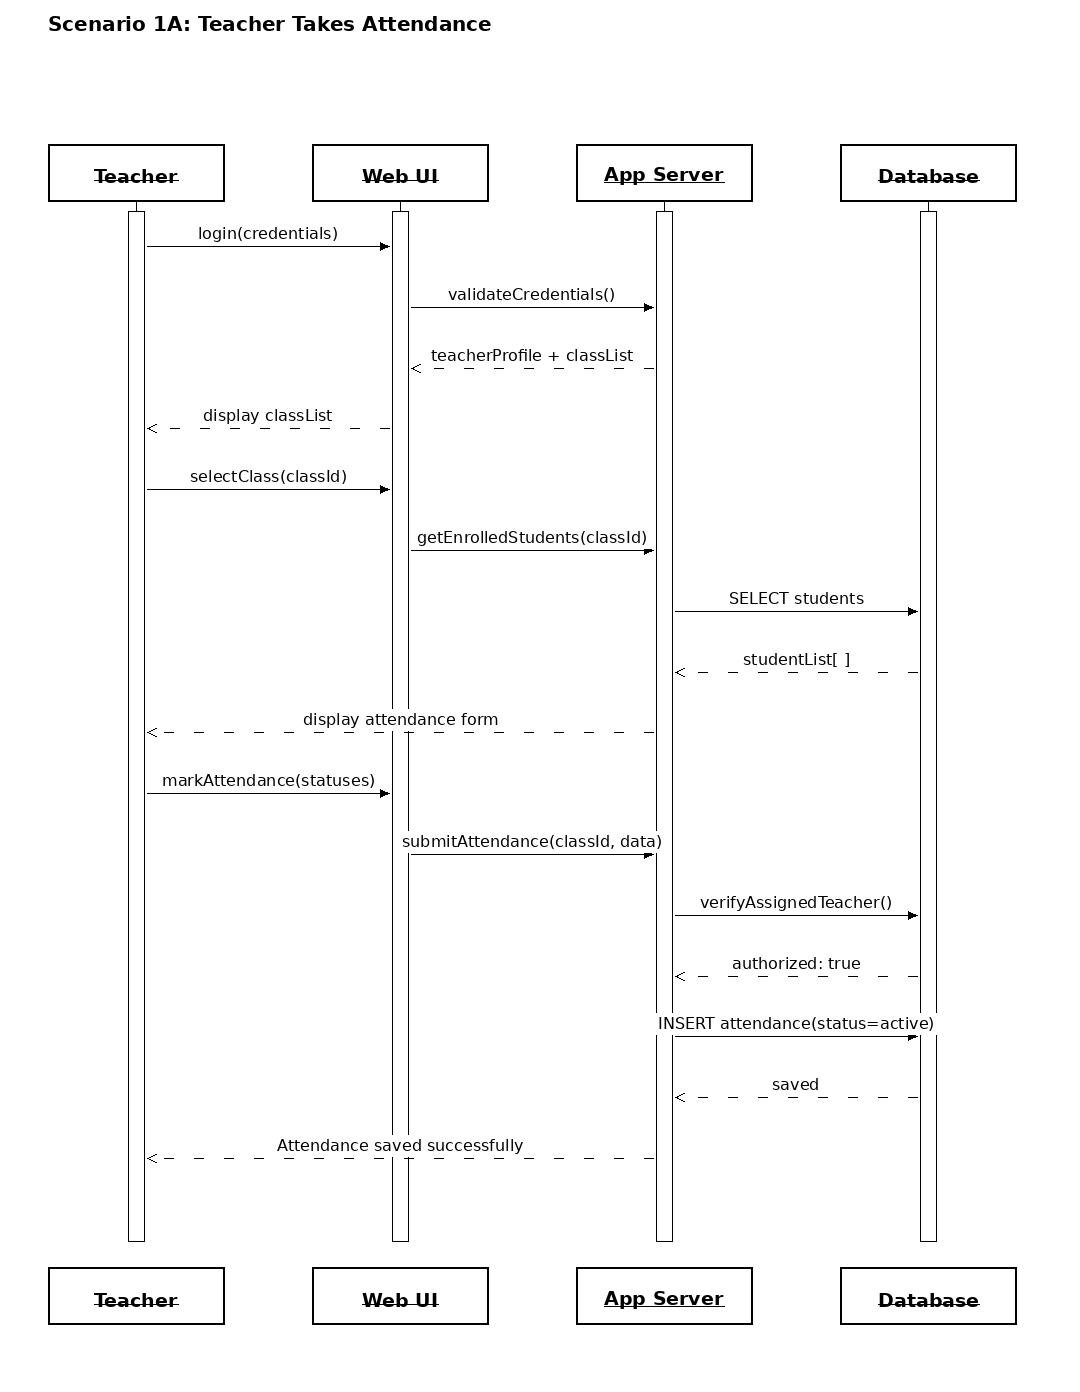
\includegraphics[width=0.5\linewidth]{figures/scenario_1a.png}
    
    \label{fig:placeholder}
\end{figure}
\begin{figure}[H]
    \centering
    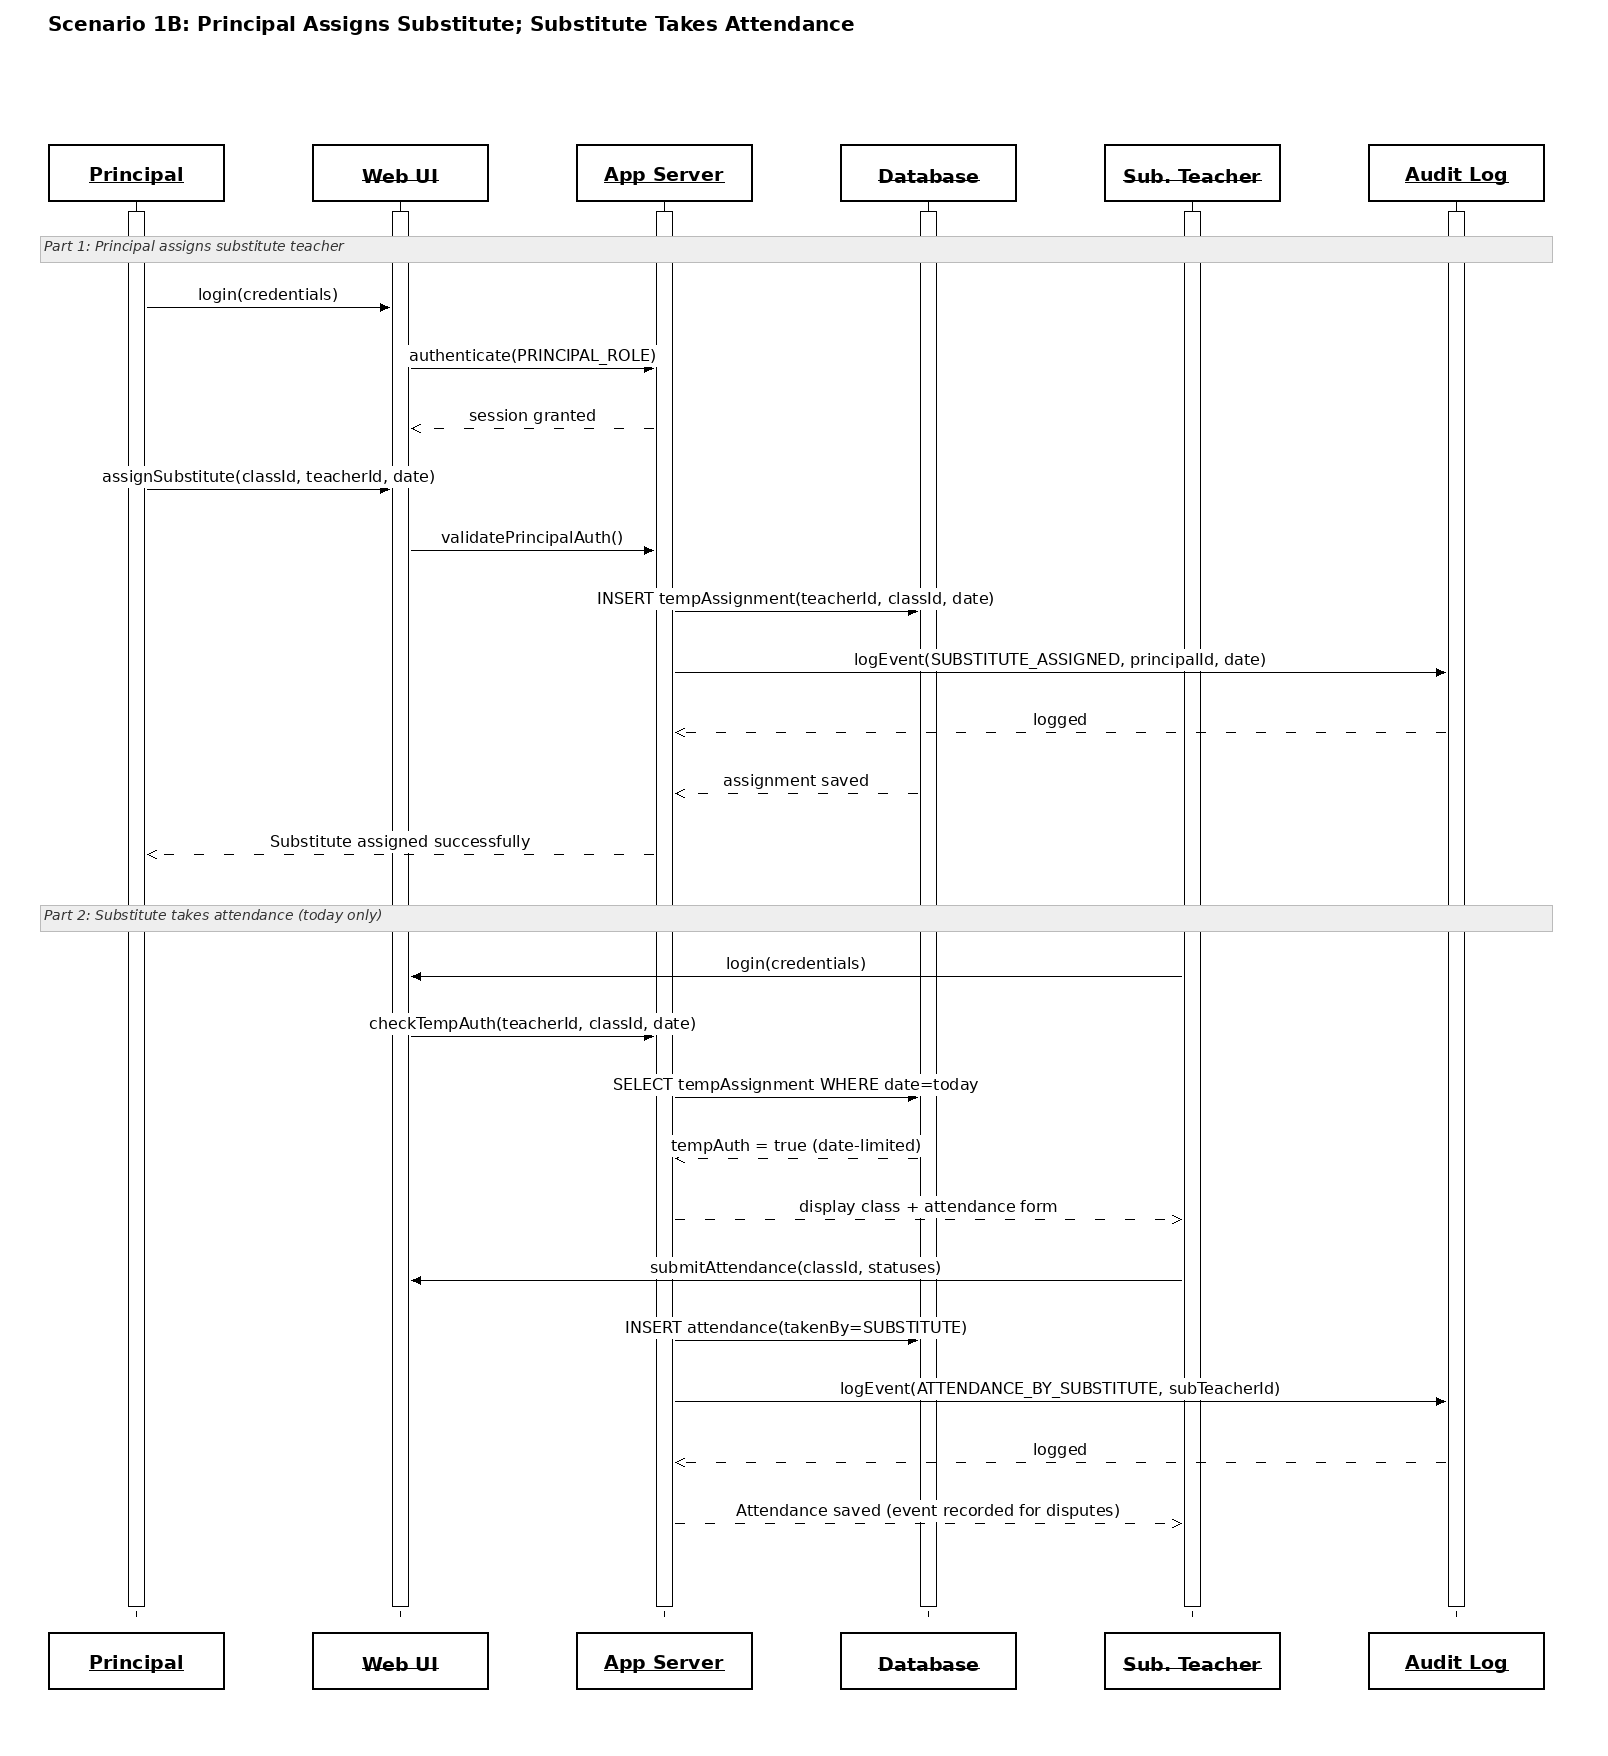
\includegraphics[width=0.5\linewidth]{figures/scenario_1b.png}
    
    \label{fig:placeholder}
\end{figure}
\begin{figure}[H]
    \centering
    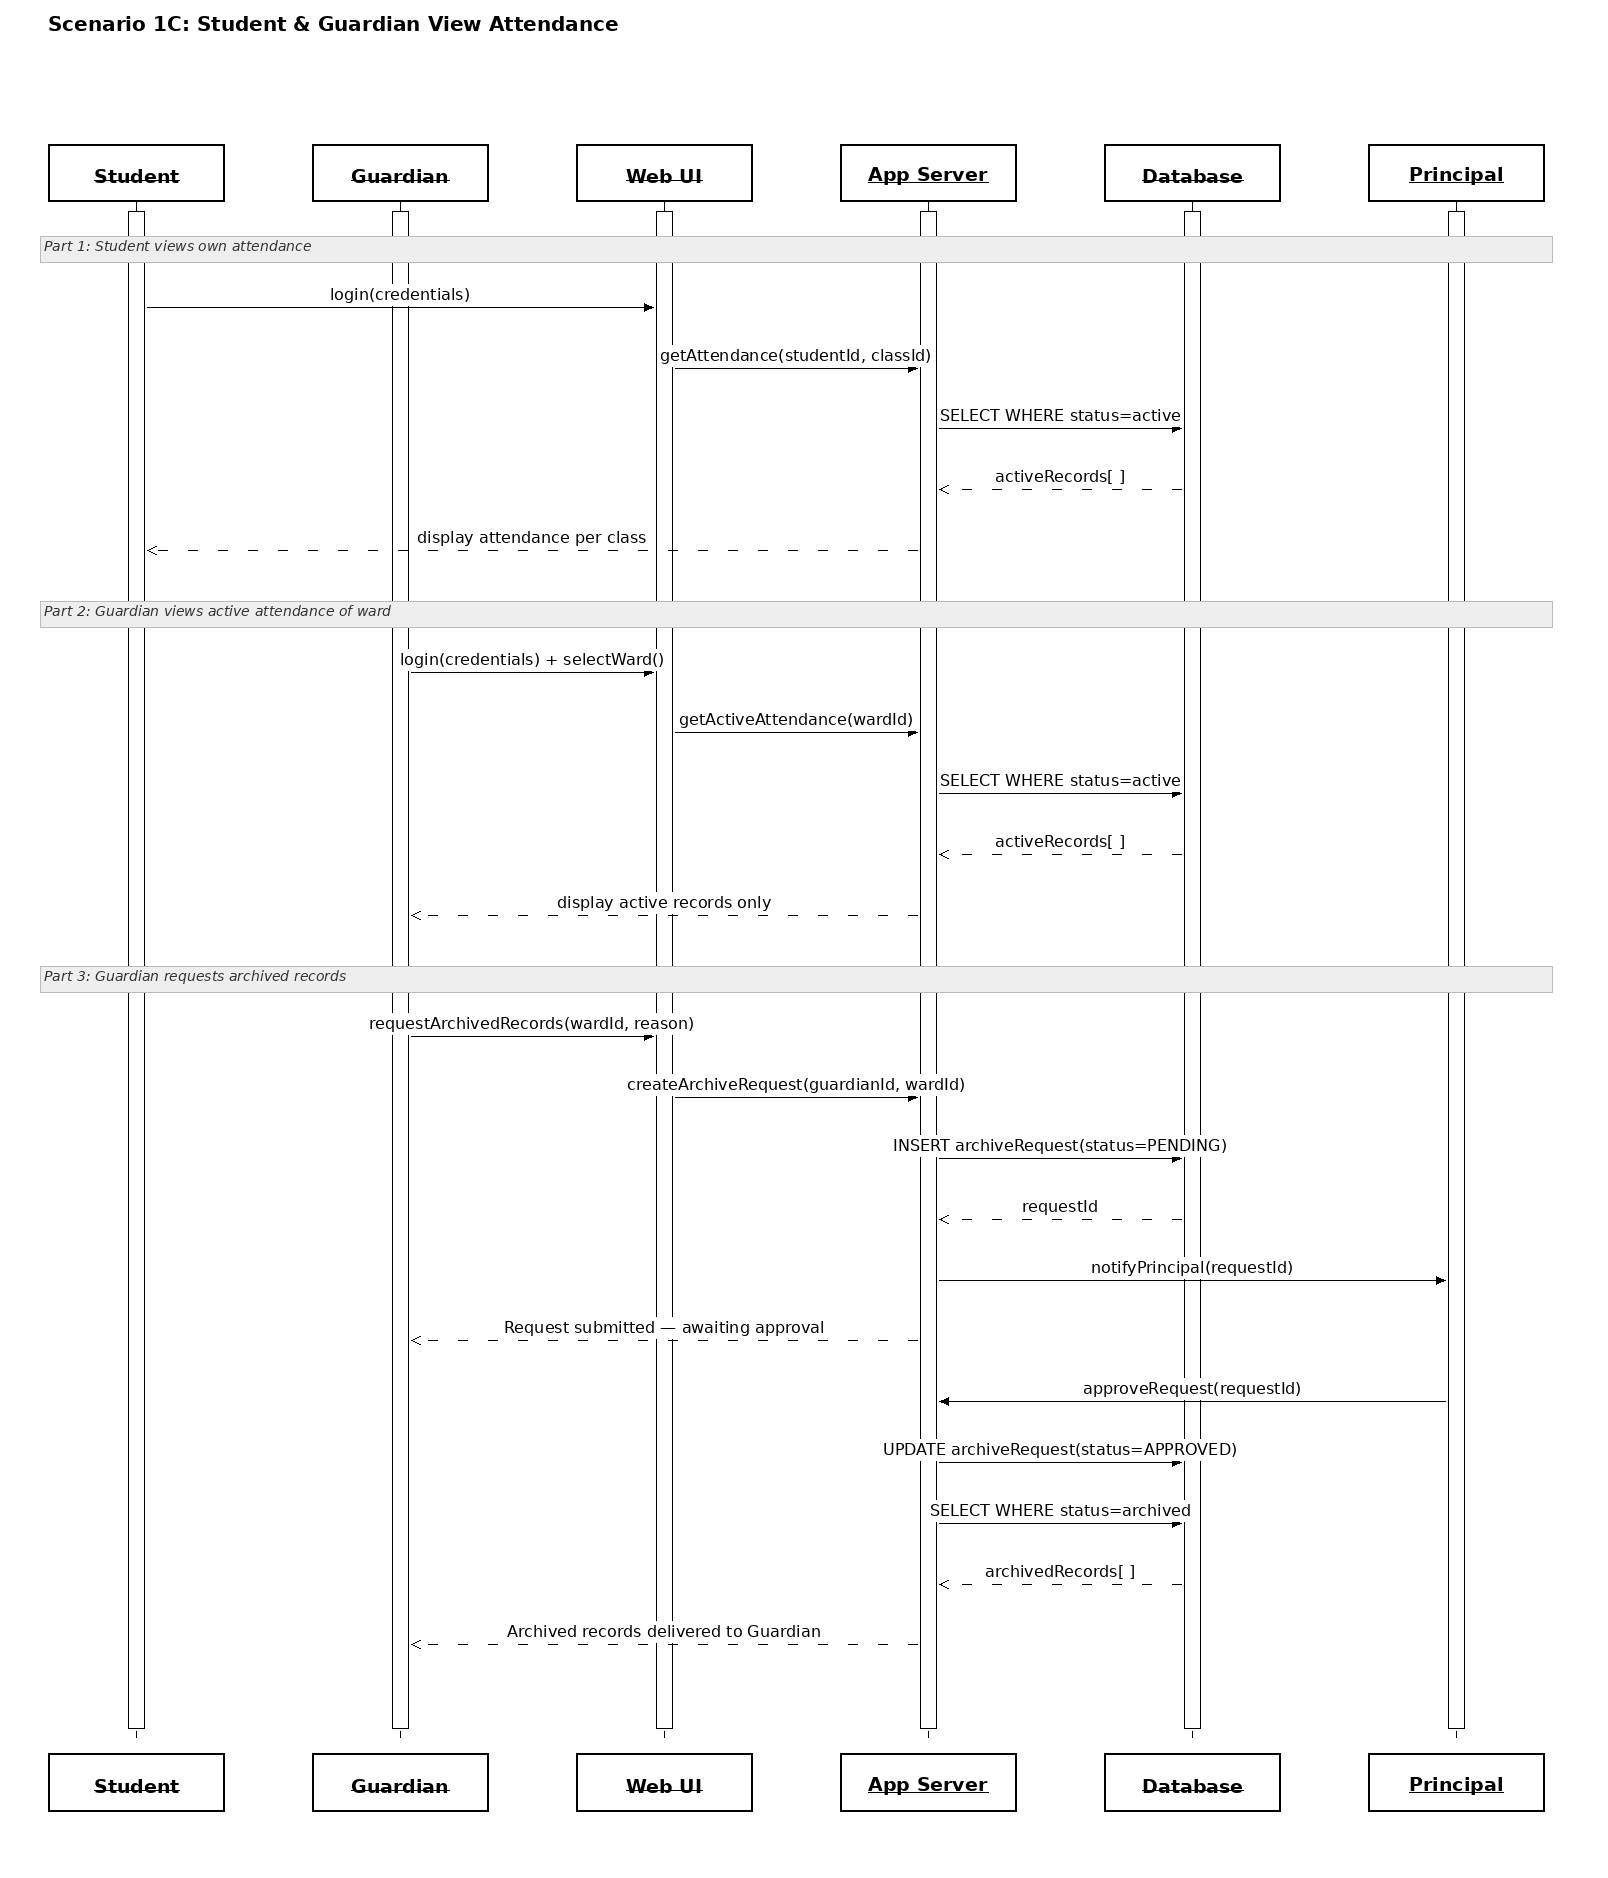
\includegraphics[width=0.5\linewidth]{figures/scenario_1c.png}
    \caption{Attendance System}
    \label{fig:placeholder}
\end{figure}
\section{Scenario 2:}
\begin{comment}
    
To give an exam, an instructor first notifies the students of the exam date and the material to be covered. She then prepares the exam paper (with sample solutions), gets it copied to produce enough copies for the class, and hands it out to students on the designated time and location. The students write their answers to exam questions and hand in their papers to the instructor. The instructor then gives the exam papers to the TAs, along with sample solutions to each question, and gets them to mark it. She then records all marks and returns the papers to the students.

Draw a sequence diagram that represents this process. Make sure to show when is each actor participating in the process. Also, show the operation that is carried out during each interaction, and what its arguments are.
\end{comment}

\begin{figure}[H]
    \centering
    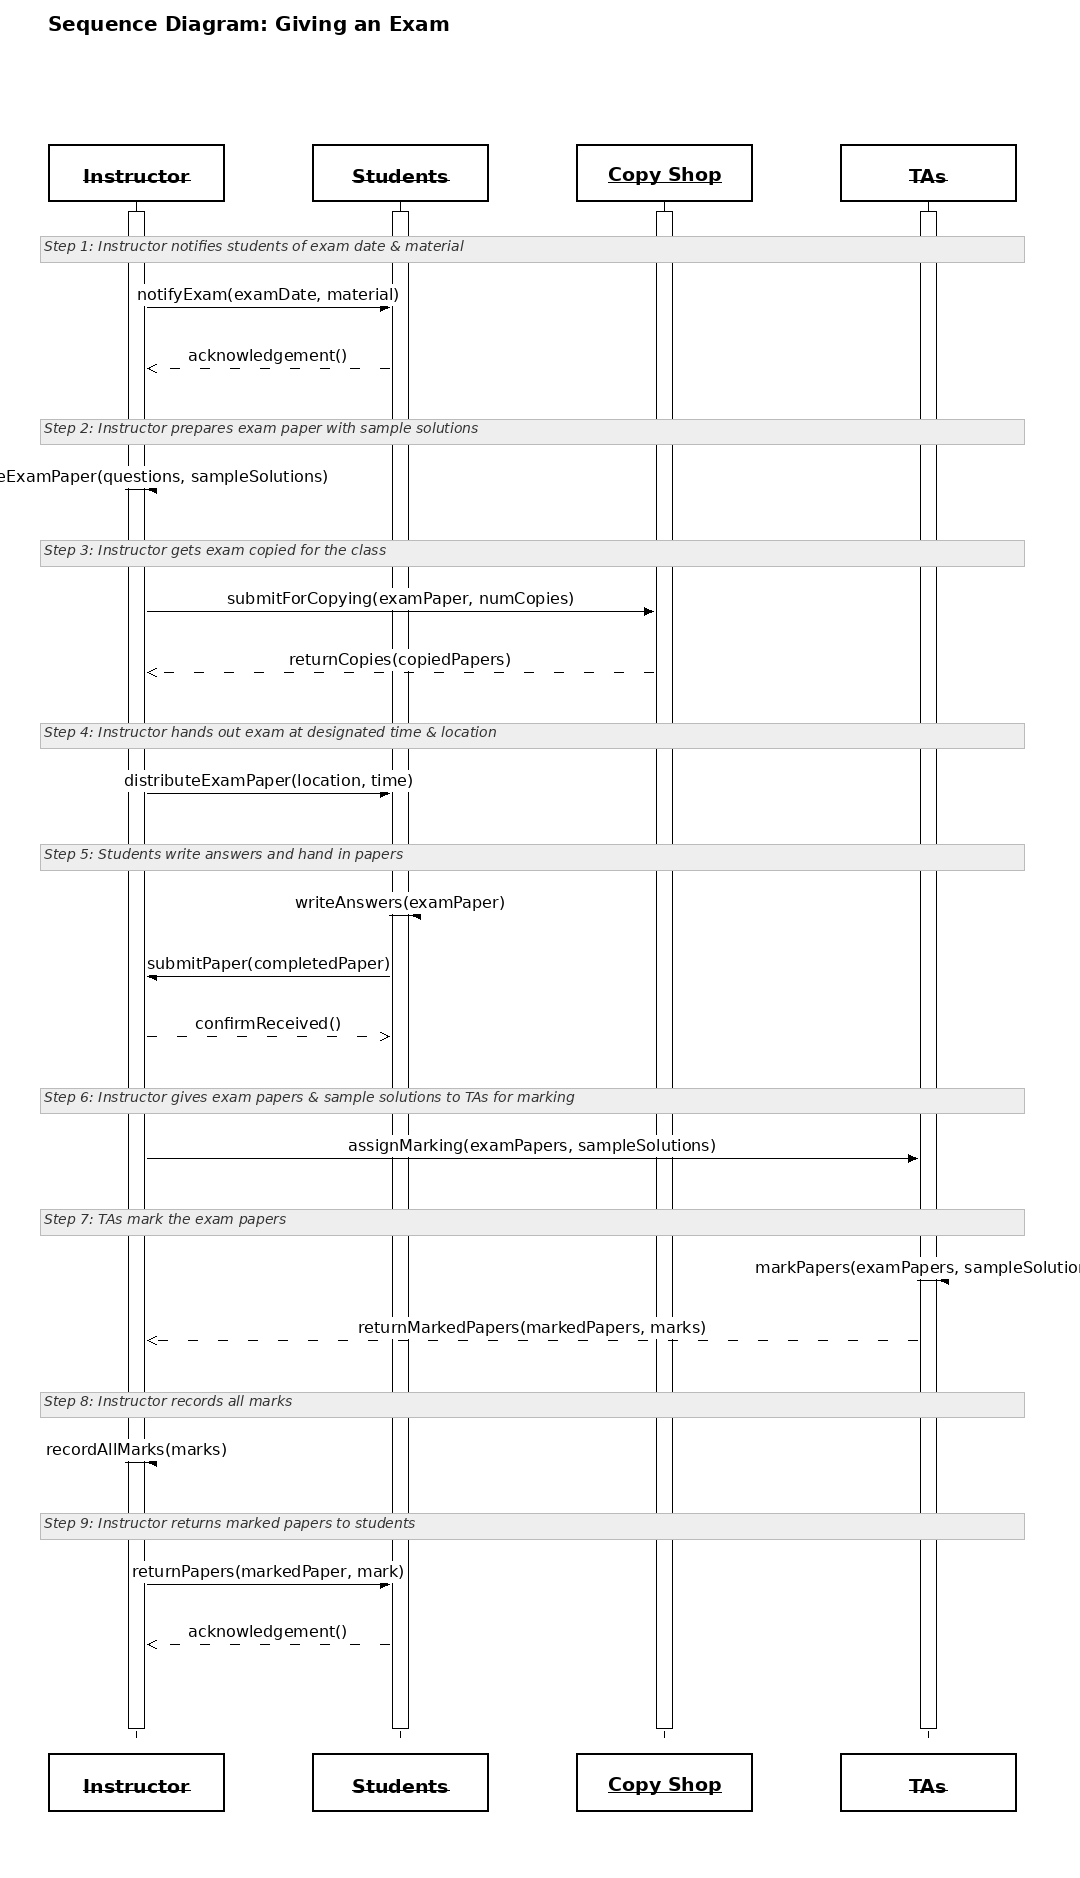
\includegraphics[width=0.7\linewidth]{figures/scenario_exam.png}
    \caption{Scenario 2: Exam System}
    \label{fig:placeholder}
\end{figure}

\section{Scenario 3:}
\begin{comment}
    
pringfield University offers a number of courses. A course contains a number of units.
Students enrol and elect a set of units every semester. Students are allowed to enrol in a
maximum of 5 units in any given semester. They can only be enrolled into a single course at
any given point in time. However over a student’s lifetime, they may undertake a number of

different courses. Each unit has a set fee that is set at the start of the semester. This fee is to be
paid up-front in full by the students once enrolled. Some units have pre-requisite unit
requirements. Some units have co requisite unit requirements. To be enrolled in some courses,
you must have completed a certain course (e.g. to enrol into a Postgraduate course, you must
have an Undergraduate degree)
\end{comment}

\begin{figure}[H]
    \centering
    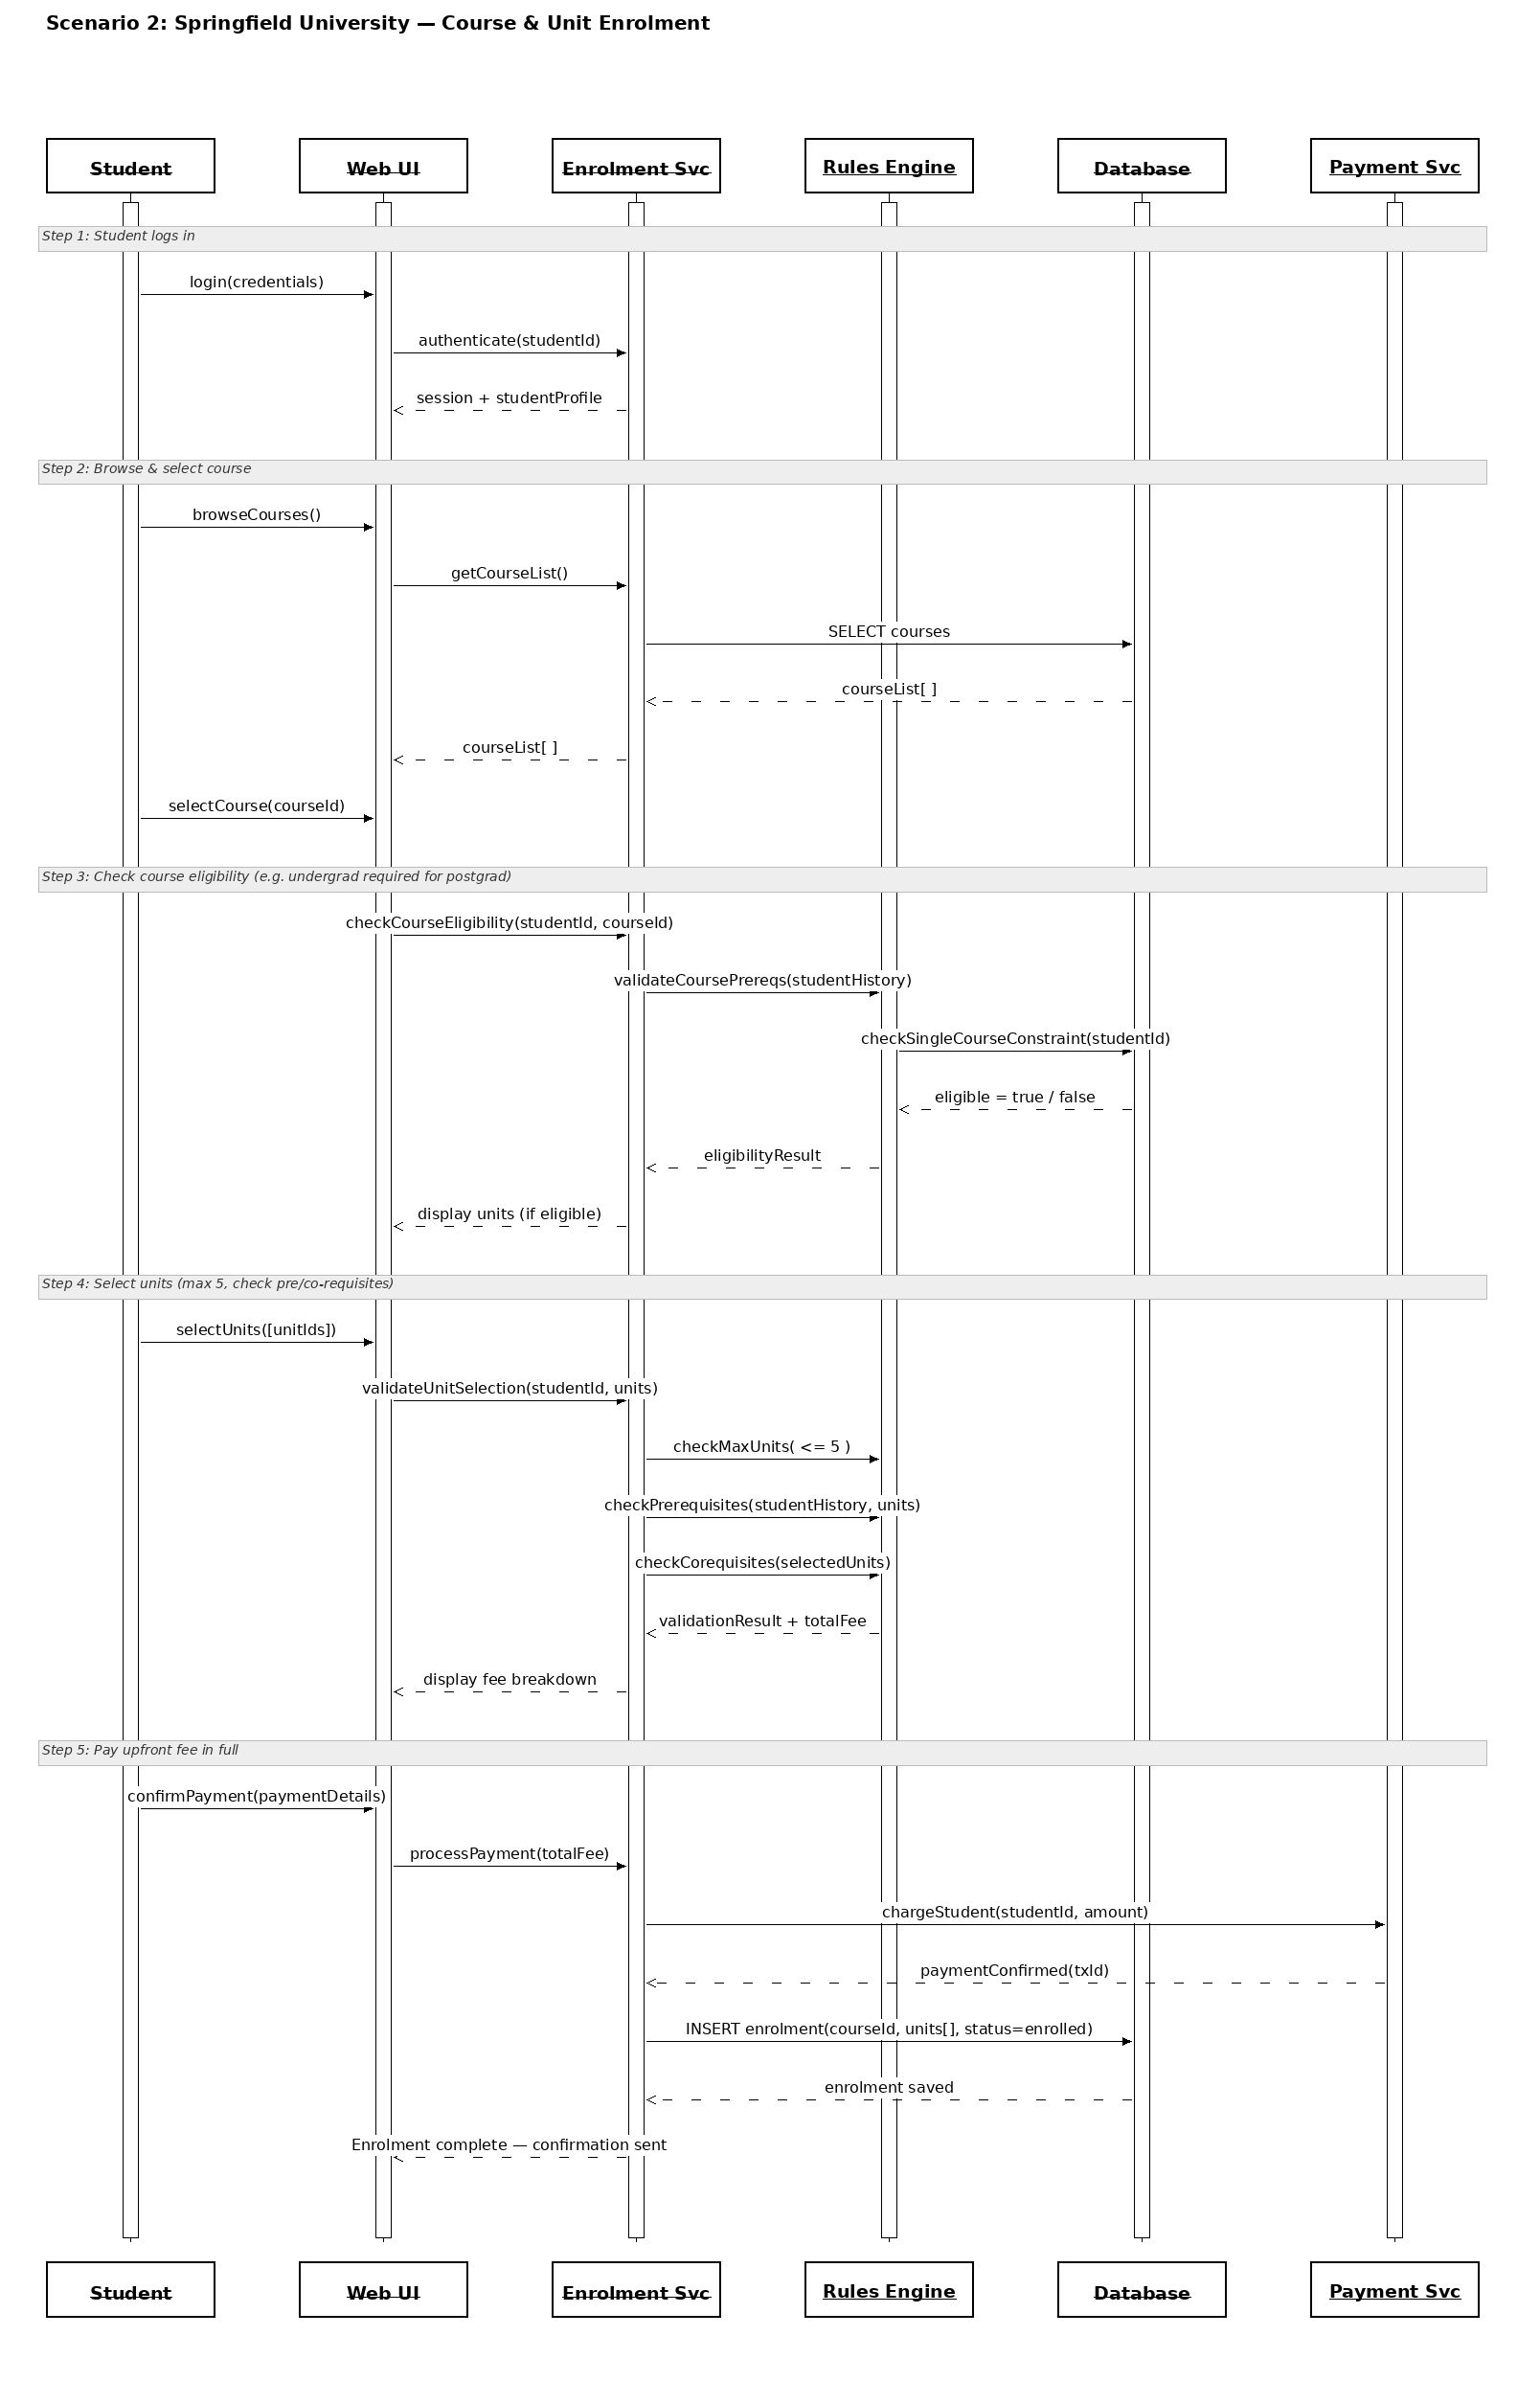
\includegraphics[width=0.7\linewidth]{figures/scenario_2.png}
    \caption{Course Enrolling}
    \label{fig:placeholder}
\end{figure}

\section{Scenario 4:}

\begin{comment}  
Paragraphs Corporation sells books and CDs using through online shopping. The customer
adds items to her shopping cart. She may remove items or go to the check-out to make her
purchases at any time. The customer reviews her purchases, chooses a payment method and
pays. A sales employee at Paragraphs Corporation gets the order and purchase confirmation
from the system, and sends the electronic order to the warehouse. The warehouse employee
updates the order status. The customer may check the order status.
\end{comment}

\begin{figure}[H]
    \centering
    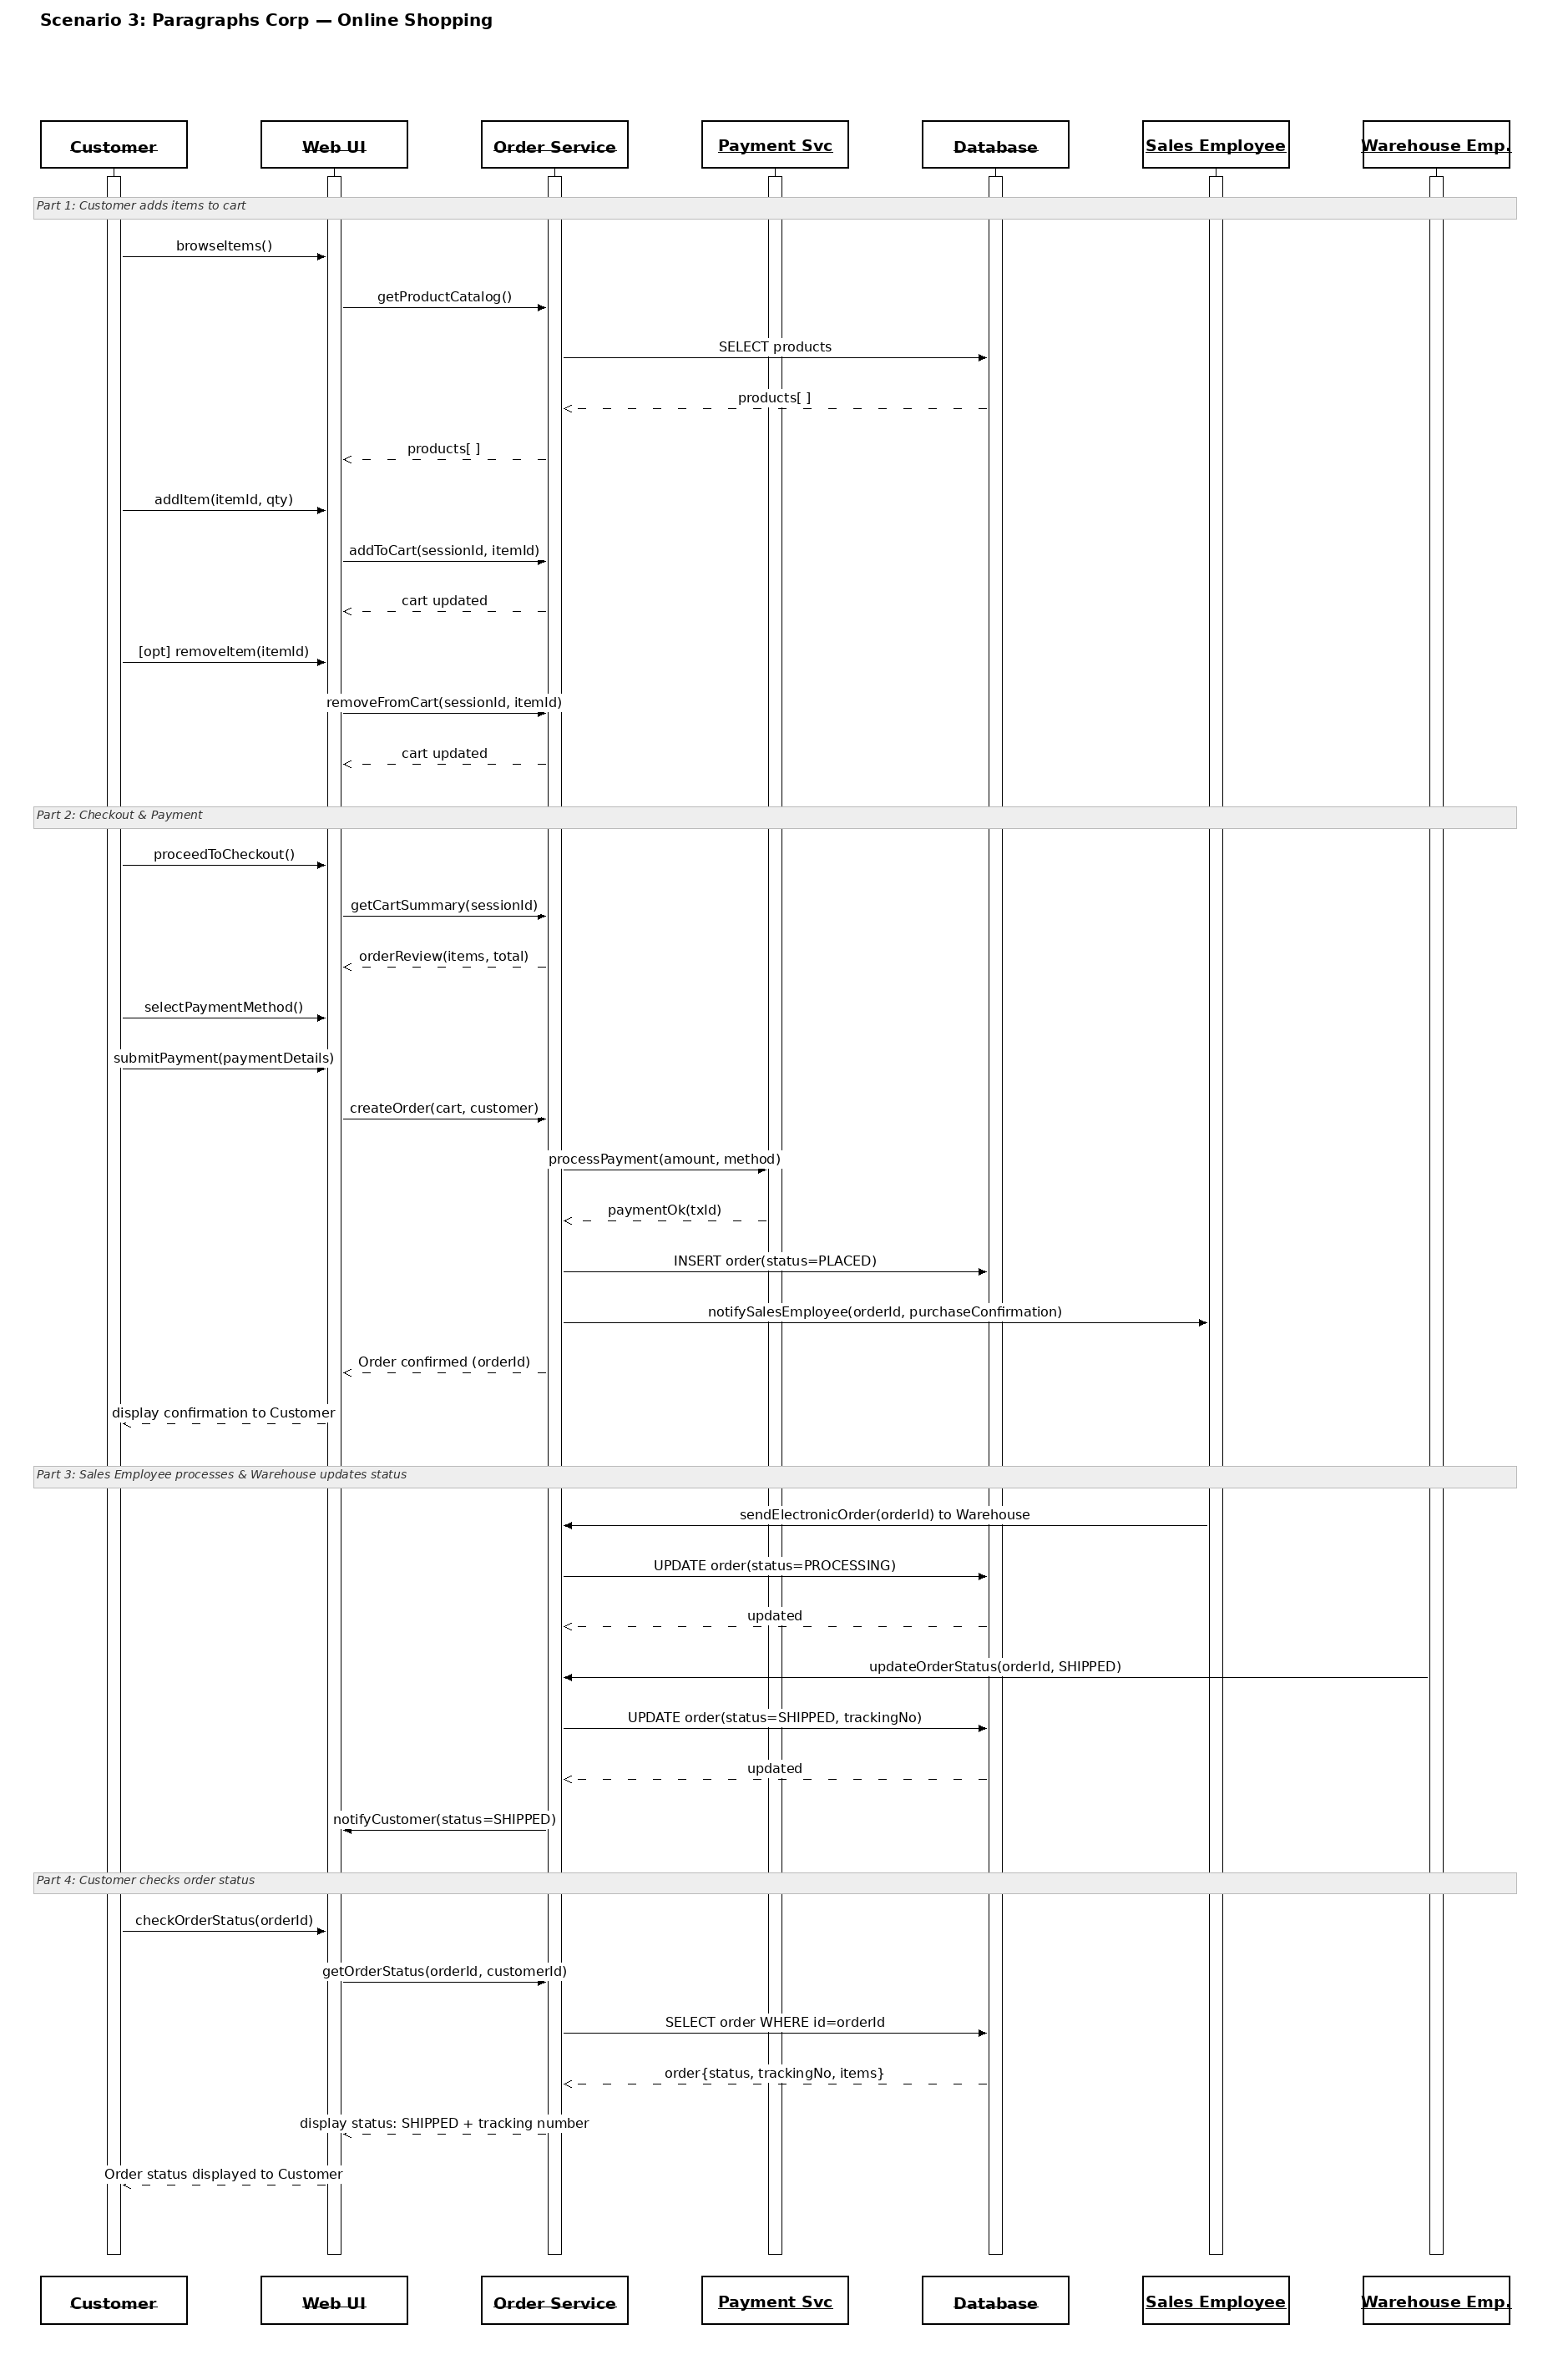
\includegraphics[width=0.7\linewidth]{figures/scenario_3.png}
    \caption{Online Shopping}
    \label{fig:placeholder}
\end{figure}